\begin{figure}[t]
\centering
  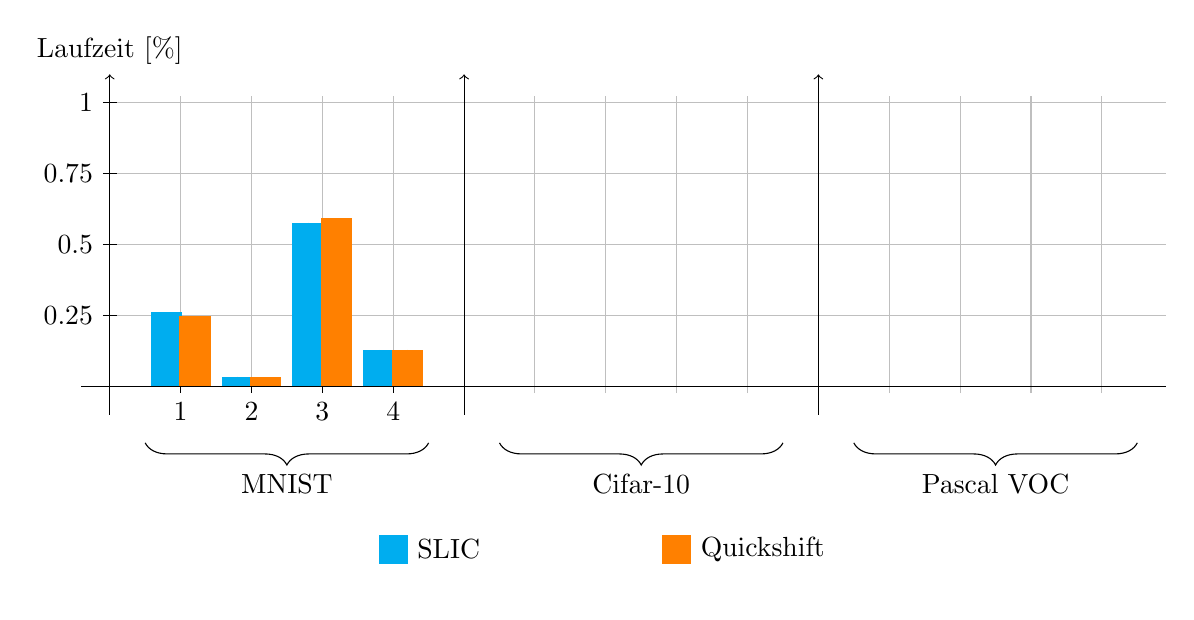
\begin{tikzpicture}[scale=0.9]
  \tikzstyle{slic}=[color=cyan, fill=cyan]
  \tikzstyle{quickshift}=[color=orange, fill=orange]

  \fill[white] (0, -2.9) rectangle (1, -1) node {};  % Abstand nach unten

  \draw[color=lightgray] (-0.1, -0.1) grid (14.9, 4.1);

  \draw[] (-0.4, 0) -- (14.9, 0);
  \draw[->] (0, -0.4) -- (0, 4.4) node[above] {Laufzeit [\%]};
  \draw[->] (5, -0.4) -- (5, 4.4);
  \draw[->] (10, -0.4) -- (10, 4.4);

  \draw (0.1, 1) -- (-0.1, 1) node[left] {$0.25$};
  \draw (0.1, 2) -- (-0.1, 2) node[left] {$0.5$};
  \draw (0.1, 3) -- (-0.1, 3) node[left] {$0.75$};
  \draw (0.1, 4) -- (-0.1, 4) node[left] {$1$};

  \draw[slic,       line width=0.4cm] (0.8, 0) -- (0.8, 1.0456);
  \draw[quickshift, line width=0.4cm] (1.2, 0) -- (1.2, 0.986);
  \draw (1, 0) -- (1, -0.1) node[below] {$1$};

  \draw[slic,       line width=0.4cm] (1.8, 0) -- (1.8, 0.1344);
  \draw[quickshift, line width=0.4cm] (2.2, 0) -- (2.2, 0.1224);
  \draw (2, 0) -- (2, -0.1) node[below] {$2$};

  \draw[slic,       line width=0.4cm] (2.8, 0) -- (2.8, 2.3084);
  \draw[quickshift, line width=0.4cm] (3.2, 0) -- (3.2, 2.3674);
  \draw (3, 0) -- (3, -0.1) node[below] {$3$};

  \draw[slic,       line width=0.4cm] (3.8, 0) -- (3.8, 0.5116);
  \draw[quickshift, line width=0.4cm] (4.2, 0) -- (4.2, 0.5148);
  \draw (4, 0) -- (4, -0.1) node[below] {$4$};

  \draw [decoration={brace,mirror,amplitude=8pt},decorate] (0.5,-0.8) -- node[below=8pt] {MNIST} (4.5,-0.8);

  \draw [decoration={brace,mirror,amplitude=8pt},decorate] (5.5,-0.8) -- node[below=8pt] {Cifar-10} (9.5,-0.8);

  \draw [decoration={brace,mirror,amplitude=8pt},decorate] (10.5,-0.8) -- node[below=8pt] {Pascal VOC} (14.5,-0.8);

  \tikzstyle{node}=[rectangle,draw, minimum width=10pt, minimum height=10pt, inner sep=0pt]
  \node[node, slic,       label=right:\gls{SLIC}] (1) at (4, -2.3) {};
  \node[node, quickshift, label=right:Quickshift] (2) at (8, -2.3) {};
\end{tikzpicture}

\begin{tabular}{ll}
  \toprule
  1. Segmentierung & 2. Adjazenzbestimmung\\
  3. Graphvergröberung & 4. Merkmalsextraktion\\
  \bottomrule
\end{tabular}

\caption[]{}
\label{fig:laufzeit_pipeline}
\end{figure}
